\documentclass[fyp]{socreport}

% %\usepackage{ctex}
%\usepackage[center]{titlesec}%章节标题位置
% \usepackage[BoldFont,SlantFont,CJKchecksingle]{xeCJK}

\usepackage{threeparttable}
\usepackage{booktabs}
\usepackage{graphicx}

\usepackage{amsmath}
\usepackage{amsfonts}
\usepackage{bm}%bold form in math environment
 %\sideset{}{}\sum  求和符号左上角,右上角添加标记
\usepackage{graphicx}
\usepackage{wrapfig}
\usepackage{subfigure}%多图共用caption
%\usepackage[version=3]{mhchem} %化学式  \ce{*} 见数字均为下标
% \usepackage[CJKbookmarks,bookmarksnumbered,
%                      bookmarksopen,colorlinks,citecolor=blue,
%                      linkcolor=blue]{hyperref}%链接样式
\usepackage{geometry}
\usepackage{fontspec,xunicode,xltxtra}
\usepackage{titlesec}
\usepackage{indentfirst}
\usepackage{multicol}
\usepackage{amssymb}
\usepackage{amsthm}
%\usepackage{mathabx}
\usepackage{multirow}
\usepackage{diagbox}
%\usepackage{fixltx2e}%解决caption中使用向量的问题配合命令\MakeRobust{\overrightarrow}
%\usepackage{exercise}
\usepackage{fancyhdr}
\usepackage{titling}%调整title
\usepackage{tabu,tikz}
\usepackage{setspace} 
\usepackage{pdfpages} %insert pdf
\usepackage{textcomp} %support other codes
\usepackage{listings} %codes support
\usepackage{xcolor}
\usepackage{url}
%\usepackage{blindtext}%?
%\usepackage[svgnames]{xcolor} % Required to specify font color

% \XeTeXlinebreaklocale "zh"
%\XeTeXlinebreakskip = 0pt plus 1pt minus 0.1pt
\geometry{top=25mm,bottom=20mm,left=30mm,right=30mm}%调整正文上下边距
\chead{\zhongsong 华中科技大学本科生毕业设计(论文)开题报告}                                                                                                
\renewcommand{\headrulewidth}{1pt}  %页眉线宽,设为0可以去页眉线
\lhead{}%页眉左边
\rhead{}%页眉右边
%\oddsidemargin=11mm
%\evensidemargin=5mm
\setCJKmainfont{SimSun}
\setCJKmonofont{SimSun}
\setmainfont{Times New Roman}
\fontsize{10.5pt}{15.7pt}\selectfont
\graphicspath{{Titlepage/}{Sect1/}{Sect2/}{Sect3/}{Sect4/}}
%\numberwithin{equation}{section}

\pagestyle{fancy}
%-------调整表格线条粗细-------
%\newcolumntype{L}[1]{>{\vspace{0.5em}\begin{minipage}{#1}\raggedright\let\newline\\
%\arraybackslash\hspace{0pt}}m{#1}<{\end{minipage}\vspace{0.5em}}}
%\newcolumntype{R}[1]{>{\vspace{0.5em}\begin{minipage}{#1}\raggedleft\let\newline\\
%\arraybackslash\hspace{0pt}}m{#1}<{\end{minipage}\vspace{0.5em}}}
%\newcolumntype{C}[1]{>{\vspace{0.5em}\begin{minipage}{#1}\centering\let\newline\\
%\arraybackslash\hspace{0pt}}m{#1}<{\end{minipage}\vspace{0.5em}}}
%\makeatletter
%\def\hlinewd#1{%
%  \noalign{\ifnum0=`}\fi\hrule \@height #1 \futurelet
%   \reserved@a\@xhline}
%\makeatother
%--------------------------------

% \def\degree{${}^{\circ}$}
% \def\ee{\mathrm{e}}%自然对数底数
% \def\ii{\mathrm{i}}%复数单位
% \def\dd{\mathrm{d}}
% \def\pp{\partial}
% \def\z{\left}
% \def\y{\right}
% \def\ol{\overline}
% \def\ora{$\overrightarrow{}$}

%----------字体相关----------
\setCJKfamilyfont{song}{SimSun}
\newcommand{\song}{\CJKfamily{song}} 
\setCJKfamilyfont{hei}{SimHei}
\newcommand{\heiti}{\CJKfamily{hei}}
\setCJKfamilyfont{zs}{STZhongsong}
\newcommand{\zhongsong}{\CJKfamily{zs}}
\setCJKfamilyfont{kai}{KaiTi}
\newcommand{\kaishu}{\CJKfamily{kai}} 
\newfontfamily\Rom{Times New Roman}
\setlength{\baselineskip}{0em}
\newcommand{\chuhao}{\fontsize{42pt}{\baselineskip}\selectfont}     %初号  
\newcommand{\xiaochuhao}{\fontsize{36pt}{\baselineskip}\selectfont} %小初号  
\newcommand{\yihao}{\fontsize{28pt}{\baselineskip}\selectfont}      %一号  
\newcommand{\erhao}{\fontsize{21pt}{\baselineskip}\selectfont}      %二号  
\newcommand{\xiaoerhao}{\fontsize{18pt}{\baselineskip}\selectfont}  %小二号  
\newcommand{\sanhao}{\fontsize{15.75pt}{\baselineskip}\selectfont}  %三号  
\newcommand{\sihao}{\fontsize{14pt}{18pt}\selectfont}%     四号  
\newcommand{\xiaosihao}{\fontsize{12pt}{18pt}\selectfont}  %小四号  
\newcommand{\wuhao}{\fontsize{10.5pt}{15.7pt}\selectfont}    %五号  
\newcommand{\xiaowuhao}{\fontsize{9pt}{13pt}\selectfont}   %小五号  
\newcommand{\liuhao}{\fontsize{7.875pt}{\baselineskip}\selectfont}  %六号  
\newcommand{\qihao}{\fontsize{5.25pt}{\baselineskip}\selectfont}    %七
%\newcommand{\bb}[1]{\raisebox{-2ex}[0pt][0pt]{\shortstack{#1}}}% 表格中向下移动文字2ex
\renewcommand{\abstractname}{\xiaoerhao \heiti \textbf{摘~~要}}
\renewcommand{\contentsname}{\xiaoerhao \heiti \textbf{目~~录}}
\renewcommand{\figurename}{\wuhao\kaishu 图}
\renewcommand{\tablename}{\wuhao\kaishu 表}
\renewcommand\refname{\sihao \song \textbf{参考文献}}
%\renewcommand{\thesubsection}{\Alph{subsection}}
\titleformat{\section}{\sihao \song \bf}{\thesection}{1em}{}
\titleformat{\subsection}{\xiaosihao \song \bf}{\thesubsection}{1em}{}
%\MakeRobust{\overrightarrow}%解决caption中使用向量的问题配合命令\usepackage{fixltx2e}
%\MakeRobust{\vv}
%
%\makeatletter
\def\fnum@figure#1{\figurename\nobreakspace\thefigure\hspace{1em}}% 去掉图后面的冒号并加空白空1em
\def\fnum@table#1{\tablename\nobreakspace\thetable\hspace{1em}}% 去掉表后面的冒号并加空白1em
%\makeatother

\hypersetup{colorlinks=false,pdfborder=0 0 0} 
%\setcounter{tocdepth}{2}

%\setlength{\droptitle}{-4em}     % Eliminate the default vertical space
%\addtolength{\droptitle}{-20mm}



\usepackage{threeparttable}
\usepackage{booktabs}
\usepackage{graphicx}
\usepackage{multirow}
\usepackage{titlesec}
\usepackage{enumitem}

\usepackage{amsmath}

\usepackage[colorlinks,linkcolor=black]{hyperref}


\usepackage{fullpage}
\begin{document}
\pagenumbering{roman}
\title{A BERT-Based Framework for Targeted Sentiment Analysis}
\author{Xiang Pan}
\projyear{2020/04}
\projnumber{CP3106}


\advisor{Prof. Lee Wee Sun}
\deliverables{
	\item Report: 1 Volume
	\item }
	% \item Source Code: 1 DVD}
\maketitle
\begin{abstract}
In the report, we distinguish the differences between the general sentiment analysis and Targeted Sentiment Analysis. Further more, we analyzed the existing problems of Targeted Sentiment Analysis. To address those problems, we proposed a new BERT-based framework to solve the targeted sentiment analysis problem. Based on the framework, we introduce some auxiliary training methods to improve the accuracy of the results. To illustrate the existing methods' robustness problem toward new (unseen) targets, we introduce a new data set setting, which explicitly makes the targets in the training set and test set to be different. Then, we use the adversarial training methods to enhance the robustness of our framework training. Overall, our framework reach the performance of the state of the art in the traditional targeted sentiment analysis setting and showed robustness in the new re-split data set setting. Finally, we describe future work in targeted sentiment analysis.


% \begin{descriptors}
%     \item C5 Computer System Implementation
% 	\item G2.2 Graph Algorithms
% \end{descriptors}
\begin{keywords}
	Targeted Sentiment Analysis, Robustness, BERT, Adversarial Training, Auxiliary Training
\end{keywords}
\begin{implement}
	Python, Pytorch, RTX 2080TI
\end{implement}
\end{abstract}

\begin{acknowledgement}
   I would like to thank my friends, families, members of the laboratory and advisors.
   Without them, I would not have been able to complete this project.
   In addition, thanks to the NGNE program for giving me the opportunity to do research.
\end{acknowledgement}

\listoffigures 
\listoftables
\tableofcontents 

\chapter{Introduction}  
 

\section{Background}
In this section, we briefly discuss the history and background of the targeted sentiment analysis problem.  A detail literature survey is presented in 
Chapter \ref{ch:related}.

Sentiment analysis (also known as opinion mining) refers to methods such as identifying and extracting subjective information in the original material. Generally speaking, the purpose of sentiment analysis is to find out the attitude of the speaker or the author on certain topics or against the bipolar views of a text. This attitude may be his or her personal judgment or evaluation, or his emotional state at the time (the author ’s emotional state when making this speech), or the author ’s intentional emotional communication (that is, the author wants the reader to experience Emotions)


\section{The Problem}
In different papers, the problem has different names. The target sentence analysis is a task with several subtasks, such as target term extraction, target term sentiment classification. In this work, we focus on the target term sentiment classification.


\cite{pei2019targeted} proposed a detailed classification for the target sentiment analysis: 
We denote the $f_{cls}$ as the classification model.

Target-grounded Aspect-based Sentiment Analysis (TG-ABSA):

\begin{equation}
    f_{cls}(sentence,aspect\ terms\ related\ to\ a\ aspect category) =sentiment
\end{equation}

Targeted Non-aspect-based Sentiment Analysis(TN-ABSA)

\begin{equation}
f_{cls}(sentence,target)=sentiment
\end{equation}\label{TSA_definition}



\begin{table*}
    \centering
    \caption{Categorization of the data}
    \label{tab:autometrics}
    {\small
    \begin{tabular}{@{}l|p{0.72in}|c|c|c|c|p{0.8in}}
    \toprule
    Task & Dataset & Coherence  & Source & Collection & Target Structure & Example application domain\\
    \hline
    TG-ABSA & SemEval 2014 & Strong & Online Review & Crawling & Aspect (Entity) & Product, service, movie, Apps   \\
    TN-ABSA & Twitter & Weak & Twitter & Filtering & Entity & Event, people, organization   \\
    T-ABSA & Sentihood, Baby Care & Moderate & Forum& Crawling & (Entity, Aspect) & product, service   \\
    \bottomrule
    \end{tabular}
    }
    \end{table*}

For a general TSA task, or more precisely, target entity sentiment classification(we use TSA to illustrate in the subsequent paper), we adopt the \ref{TSA_definition} definition as our task setting and treat the aspect entity as the target term, which is also a general setting.

\section{Our Contributions}
Our Contributions is mainly on three aspects:
\begin{enumerate}
    \item A general framework for target sentiment analysis
    \item Auxiliary training methods for TSA
    \item Proposing a new robustness test setting
    \item Adversarial training methods for model's robustness towards new(never appeared in training) targets.
\end{enumerate}


\chapter{Related Work}
\label{ch:related}
\section{Text classification}
The text classification is a traditional application of NLP. As a typical sequence data format, various sequence models have been applied to the text classification problem. 



\section{Pre-trained Language models}
\begin{figure}[h]
    \centering
    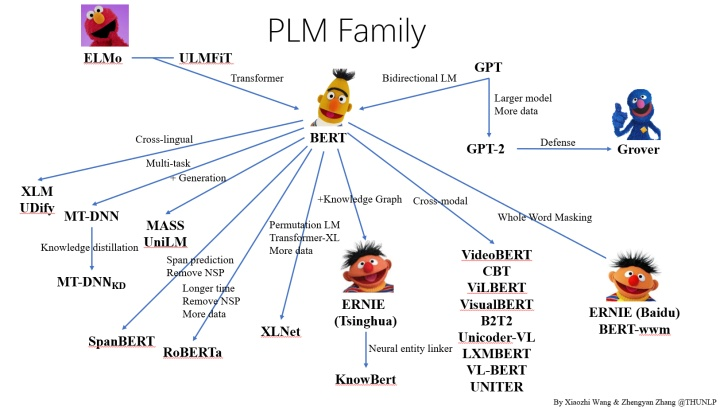
\includegraphics[width=0.7\linewidth]{./image/PLM.jpg}
    \caption{Pre-trained Language Models Family}
  \label{example}
\end{figure}

In order to perform the downstream tasks of natural language processing, it is usually necessary to represent the original text to some features. From the early statistical language model to the model based on neural networks in recent years, it is to achieve this goal. Starting from word2vec, how to learn a reasonable word vector representation has become the key to different downstream tasks. The pre-training model is trained through reasonable structure design and large-scale corpus training, so as to obtain a more general word vector representation. Using these word vectors, many NLP downstream tasks can be performed. However, due to the different corpus domains and language domain differences, the task corpus needs to be used to fine-tune the model. At the same time, due to different downstream tasks, the use of word vectors is strictly related to downstream models.

BERT \cite{devlinBERTPretrainingDeep2019} as a typical and successful pre-trained model for various NLP tasks can be seen as a baseline.  How to use the pre-trained language model to adapt to various downstream tasks and the efficient fine-tuning is focused by researchers.

\section{Aspect Based Sentiment Analysis}
We briefly review the related work in ABSA.

Using the Memory Network architecture \cite {Tang2016}, which uses a memory network to remember contextual words and explicitly model attention to target words and context.
It was found that compared with the previous model \cite {Tang2015} that used the left or right context alone, making full use of context words can improve its model.

The Attention Encoder Network (AEN) \cite {ArxSong} was tested using GloVe word vectors as input word vector representations and BERT as word vectors representation word vector representations (AEN-BERT) (a modification of the transformer architecture). The author divides the Multi-Headed Attention (MHA) layer into the MHA inner layer and MHA outer layer in order to model the target words and context differently. Such a structure is lighter than the transformer architecture.

Graph Convolutional Neural Network (GCN) \cite {ArxZhaoa2019} achieves another recent performance improvement, using graph convolutional neural network to explicitly establish the dependence between sentiment words in sentences with multiple aspects. They show that if there are multiple aspects in a sentence, the performance of their model's architecture will be particularly good.

However, the designs of architecture in these works utilize various characteristics of targeted sentiment analysis. It is hard to unify to a generic format to combine those designs for further improvement. For a more generic framework and better utilize the powerful pre-trained language models, we proposed our framework.




\chapter{Problem and Algorithm}
\section{Formal Description of Problem}
Given a text sequence with n words text=$\{w_1,w_2,w_3,w_4,...,w_n\}$ and a target with m words, target text=  $\{t_1,t_2,...,t_m\}$ with its begin position $b$, the problem is to classify the sentiment polarity $polarity=\{positive,neutral,negative\}$ towards the given target in the context. We followed the SemEval 2014 Task 4\cite{pontiki-etal-2014-semeval} subtask 2.




\section{Design of Algorithm}
\section{BERT for Text Classification}

\paragraph{BERT for sentence text classification}


As a powerful pre-trained universal language model, BERT can be used in various downstream tasks.
To utilize bert, we have several direct ways:
\begin{enumerate}
    \item Using BERT embeddings as the input of a sequence
    \item Fine-tuned BERT by [CLS] classification token.
\end{enumerate}

To enhance the performance, \cite{sun2019finetune} proposed several methods for text classification: 


\paragraph{Trick for text classification}

\begin{enumerate}
    \item Various fine tuning methods
    \begin{enumerate}
        \item Within-task pre-training
        \item In-domain pre-training
        \item Cross-domain pre-training
    \end{enumerate}
    
    \item Different learning rates are used for different layers of Bert
\end{enumerate}


Those methods only consider the sentence-level classification. For TSA, the classification problem is more fine-grained, hence we will introduce our BERT-based framework for TSA.


\section{BERT for TSA}

As described in the related work, BERT-SPC \cite{Song2019} repeats the target words at the end of the context sentence. 

\begin{figure}[h]
    \centering
    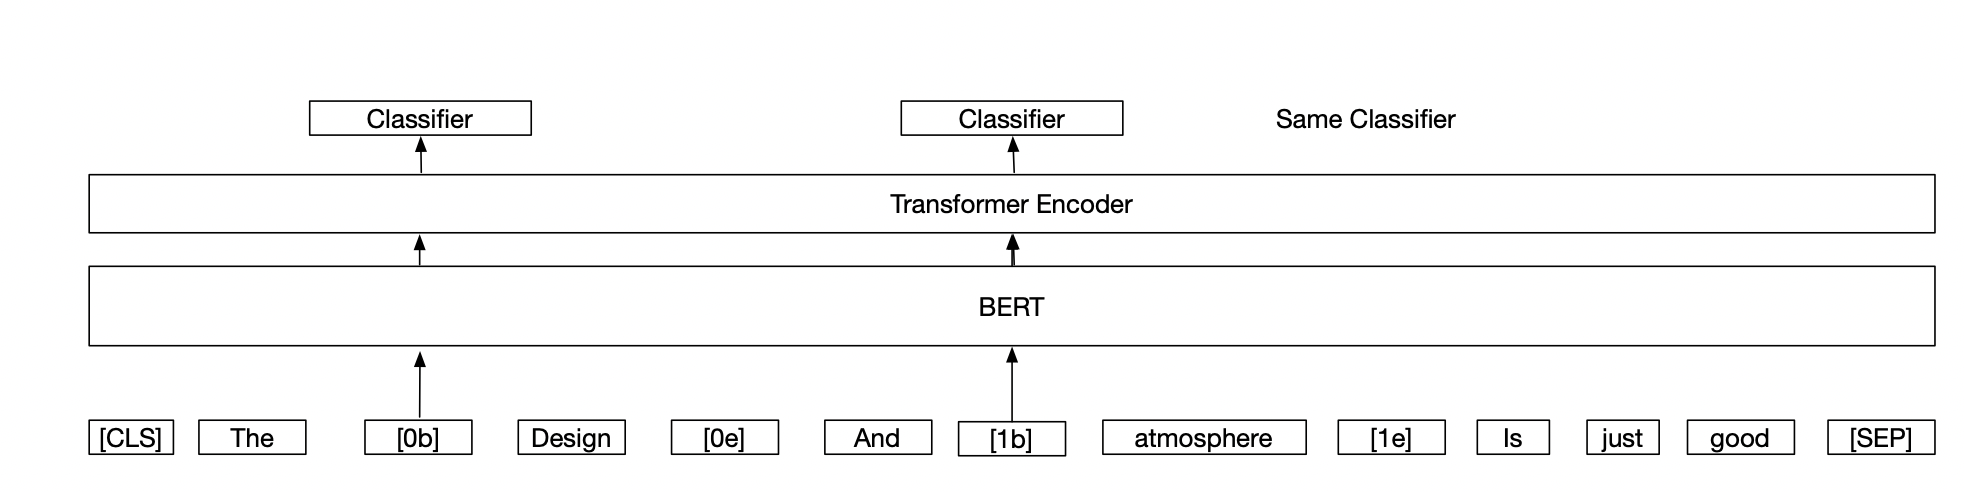
\includegraphics[width=\linewidth]{./image/Framework.png}
    \caption{Our framework for TSA}
  \label{Framework}
\end{figure}

% For original bert, the most direct way to utilize bert 

As shown in the image \ref{Framework}, we add the beginning token and end token around the target. Such an idea was inspired by the \cite{soares2019matching}, which add special tokens for relationship extraction.

To test the token add methods, in our initial experiments, we add the same token for different targets in the context sentence. However, the result is worse than only taken for the target you need to do the classification. The reason may be that BERT model can not distinguish which token should aggregate the classification information.





\section{Auxiliary training methods for TSA}

\begin{figure}[h]
    \centering
    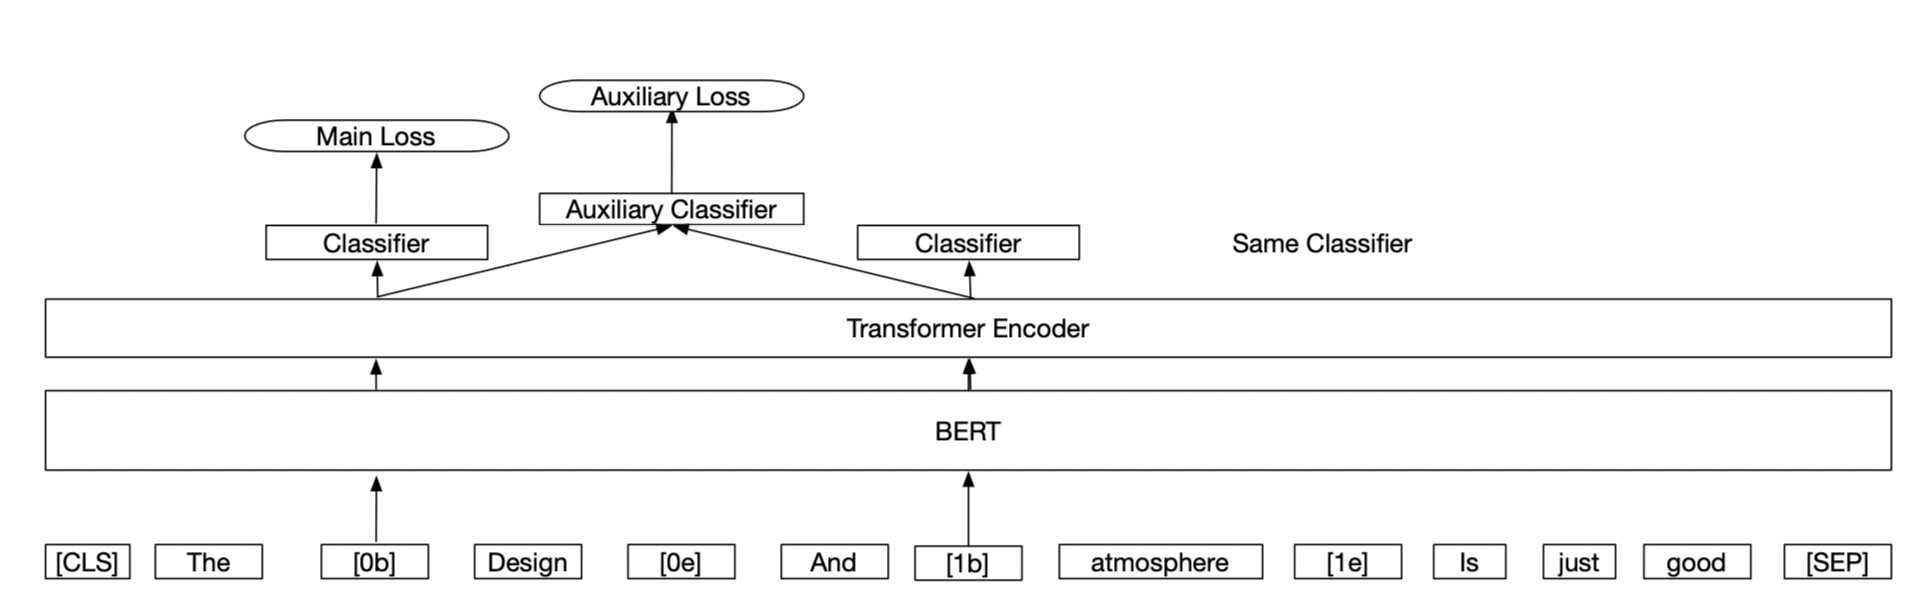
\includegraphics[width=\linewidth]{./image/aux.png}
    \caption{auxiliary training}
  \label{Framework}
\end{figure}


To enhance bert by utilizing the targets' position information and the relationship between different targets in the same sentence, we use auxiliary training methods to better fine-tune BERT.

we denote the auxiliary classification function by $f_{aux}$, the classification can be presented as:  

\begin{equation}
    f_{aux}(main\ target,other\ {target})=sentiment\ {pair}
\end{equation}

For a sentence with more than 2 targets, we iterate all the other targets in the sentence. Thus, the auxiliary loss can be denoted as:  
\begin{equation}
    loss_{aux}(main\ target)=\sum_{other\ {target_i} \in other\ {targets} }f_{aux}(main\ target,other\ {target_i})
\end{equation}





\section{Adversarial training methods for Robustness of TSA}
\cite{karimi2020adversarial} use adversarial training methods from \cite{miyato2016adversarial} to enhance BERT-PT\cite{xu2019bert} model's performance. We utilize a similar method in our framework.

\begin{figure}[h]
    \centering
    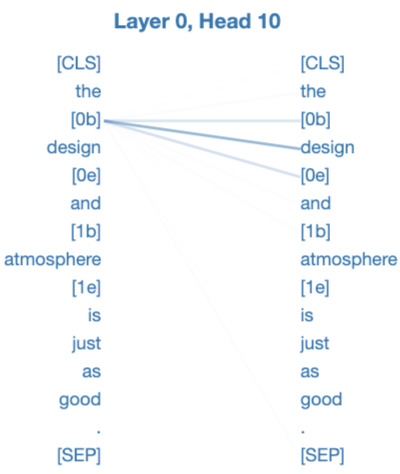
\includegraphics[width=\linewidth]{./image/target-depence.png}
    \caption{Bottom layer of BERT visualization}
  \label{target-depence}
\end{figure}

From the \ref{target-depence} we can see that our model still has some dependence on the bottom layer of BERT. Such dependence may contribute to a higher score in reappearing target sentiment analysis. However, when a target is never seen before, the dependence may decrease the robustness. We would like to make the framework to be less reliant on the target tokens.

\subsection{Robustness Test Settings}
For simplicity, we remove those samples, which own the same or similar targets in the train set, from the test set.

\begin{table}[]
    \centering
    \caption{
		Statistics of re-split dataset.\\
	}
    \begin{tabular}{llll}
    \hline
    stat-type  & train         & test &     \\ \hline
    twitter    & size          & 6248 & 619 \\ \hline
               & target-number & 104  & 358 \\ \hline
    restaurant & size          & 3608 & 393 \\ \hline
               & target-number & 606  & 304 \\ \hline
    laptop     & size          & 2328 & 282 \\ \hline
               & target-number & 461  & 232 \\ \hline
    \end{tabular}
\end{table}

\subsection{Adversarial training}
The adversarial training method searches the worst perturbations which can make the largest classification error. Towards the main optimization function, the adversarial training target is to maximize the main loss function. For maximizing the error rate, the following perturbations are added to the input embeddings to create new adversarial sentences in the embedding space. 

\begin{equation}
r_{adv} = -\epsilon \frac{g}{||g||_2}
\end{equation} 

\begin{equation}
    g = \nabla_{x}\, \log\,  p(y|x;\hat{\theta})
\end{equation} and $p_{adv}=\epsilon$ is the size of the perturbations.

\begin{center}
	$loss_{aux}=- \log p(y|x + r_{adv};\theta)$
\end{center}

For robustness test, 
The total training loss is:  
\begin{equation}
    loss(main\ target)=loss_{main}(begin\_{token})+p_{aux}*loss_{aux}(main\ target)+loss_{adv}
\end{equation}


For the hyper parameters $p_{aux}$ and $p_{adv}$ is adjusted by the experiment results.

\chapter{Evaluation}
In this section, we describe the experiment environment, evaluation details and results of our experiments.

\section{Implementation Details}

We list our experiment environment: \\
OS: Ubuntu 18.04 LTS (Bionic Beaver)\\
Kernel: x86\_64 Linux 4.15.0-70-generic2\\
Shell: zsh 5.4.2\\
CPU: Intel Xeon W-2123 @ 8x 3.9GHz\\
GPU: GeForce RTX 2080 Ti\\
RAM: 31859MiB \\




Our experiment is based on the code of \href{https://github.com/songyouwei/ABSA-PyTorch}{ABSA-Pytorch}. We release our code in \href{https://github.com/Xiang-Pan/TSA-PyTorch}{TSA-Pytorch}.

Our bert model is based on the \href{https://github.com/huggingface/transformers}{huggingface's transformers} library. For some bottom-modified, we direct modified the source code of the library, details refer to our source code.

\section{Experimental Setup}

batch-size: 32\\
optimizer: adam\\
valset-ratio: 0.05\\
max-seq-len: 128\\
num-epoch: 10(The best performance model usually trained with 2 or 3 epochs for general bert, bert-multi-target(our framework) usually takes up to 10 and adversarial training usually takes up to 10)\\

% \subsection{Targeted Sentiment Analysis}
% For our framework, the number of fine-tuning epochs is less than 10.


% \subsection{Domain Adaption' effect on Targeted Sentiment Analysis}


% \subsection{Robustness of Targeted Sentiment Analysis Algorithms}











\section{Visualization}
\subsection{Pre-trained BERT Visualization}


\begin{figure}[h]
    \centering
    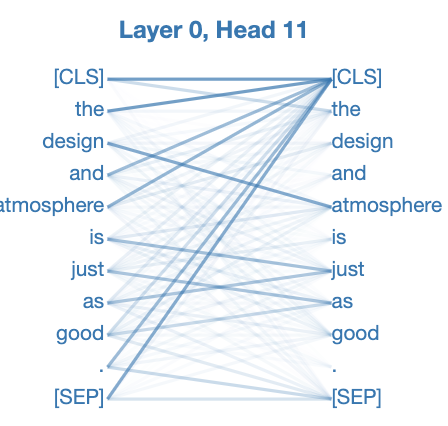
\includegraphics[width=\linewidth]{./image/L0H11.png}
    \caption{Layer 0 Head 11 of original BERT}
  \label{Framework}
\end{figure}

From the visualization, we can find that the bert\_spc model's attention is densely connected to the [SEP] token and [CLS] token. A similar structure can be found in our framework, the beginning token gives additional positional information. Thus we can enhance the model performance by using aggregate classification token embeddings.

\subsection{BERT-SPC Visualization}
We attached the full visualization of whole the bert-spc model's attention in the appendix. The bert's different attention is less modified on the fine-tuning stage. When we add an additional transformer encoder layer above the bert model, the model training is getting much easier and a little performance increases.



\section{Results}
\subsection{TSA results}
For the test results, we experiment on the original semeval \cite{pontiki-etal-2014-semeval} data set and twitter data set \cite{mitchell2013open}. For comparison, we use the reported results from TD-BERT \cite{8864964}.


\begin{table*}[h]
    \small
    \centering
    \resizebox{\textwidth}{!}{
    \begin{threeparttable}
    \caption{
		Test results on three typical data sets.
	}
      \begin{tabular}{cccccccc}
      \toprule
      \multirow{2}{*}{ }&\multirow{2}{*}{\ {Models}}&
      \multicolumn{2}{c}{\ {Twitter}}&\multicolumn{2}{c}{\ {Restaurant}}&\multicolumn{2}{c}{\ {Laptop}}\cr
      \cmidrule(lr){3-4} \cmidrule(lr){5-6} \cmidrule(lr){7-8}
      &&Accuracy&Macro-F1&Accuracy&Macro-F1&Accuracy&Macro-F1\cr
      \midrule
          \multirow{4}*{\ {RNN baselines}}
          &TD-LSTM           &0.7080&0.6900              &0.7563&-                  &0.6813&-         \cr
          &ATAE-LSTM         &-&-                        &0.7720&-                  &0.6870&-         \cr
          &IAN               &-&-                        &0.7860&-                  &0.7210&-         \cr
          &RAM               &0.6936&0.6730              &0.8023&0.7080             &\ {0.7449}&\ {0.7135}     \cr
      \midrule
          \multirow{3}*{\ {Non-RNN baselines}}
          &Feature-based SVM &0.6340&0.6330              &0.8016&-                  &0.7049&-           \cr
          &Rec-NN            &0.6630&0.6590              &-&-                       &-&-              \cr
          &MemNet            &0.6850&0.6691              &0.7816&0.6583             &0.7033&0.6409    \cr
      \midrule
          \multirow{3}*{\ {AEN-BERT}}
        %   &AEN-GloVe  &\ {0.7283}&0.6981  &\ {0.8098}&\ {0.7214}  &0.7351&0.6904 \cr
            &BERT &0.7464&0.7304 & 0.8128 & 0.6979 & 0.7654 & 0.7283\\
            &BERT-SPC  &\ {0.7355}&\ {0.7214} &\ {0.8446}&\ {0.7698} &\ {0.7899}&\ {0.7503} \cr
          &AEN-BERT &\ {0.7471}&\ {0.7313} &\ {0.8312}&\ {0.7376} &\ {0.7993}&\ {0.7631} \cr
    \midrule
        \multirow{1}*{\ {BERT-PT}}
        &BERT-PT  &-&-  &\ {0.8495}&\ {0.7696}  &0.7807&0.7508 \cr
    \midrule
        \multirow{2}*{\ {TD-BERT}}
        &TD-BERT  &0.7669&0.7428  &\ {0.8510}&\ {0.7835}  &0.7807&0.7508 \cr
        
        &TD-BERT-QA-CON  & 0.7731&0.7440  &{0.8456}&{0.7961}  &0.7842&0.7437 \cr

    \midrule
        \multirow{2}*{\ {Our}}
        &Framework  &0.7673&0.7451  &\ {0.843}&\ {0.780}  &
        0.7633&0.7291 \cr
        &Framework+aux1.0  &-&-  &\textbf{0.8554}&\textbf{0.7962}  &\textbf{0.7806}&\textbf{0.7523} \cr
        &Framework+aux0.1  &-&-  &\ {0.8464}&\ {0.788}  &0.7759&0.7370 \cr


      \bottomrule
      \end{tabular}
      \label{tab:result}
      \end{threeparttable}}
  \end{table*}

\subsection{Domain Adaption Test Results}

The result is shown on \ref{domain-res}. The domain bert is post-trained on same domain unlabeled articles. We use the domain bert from BERT-ADA\cite{alex2019adapt}.

\begin{table}[h]
    \centering
    \caption{Test results on three domain bert}
    \label{domain-res} 



    \begin{tabular}{llllllll}
    \hline
           &           & Twitter &        & Restaurant &         & Laptop &        \\ \hline
    Domain & Method    & acc      & f1     & acc         & f1      & acc    & f1     \\ \hline

    % \midrule
    % \multirow{3}*{\ {BERT-ADA}}
    joint&BERT-ADA Joint  &{-}&{-} &{0.8635}&{0.7889} &{0.7896}&{0.7418} \\ \hline
    rest&BERT-ADA Rest  &{-}&{-} &{0.8714}&{0.8005} &{0.7860}&{0.7409}\\ \hline
    lapt&BERT-ADA Lapt  &{-}&{-} &{0.8551}&{0.7809}&{0.7919}&{0.7418} \\ \hline
    

    
    \midrule
           & Framework & 0.7673   & 0.7451 & 0.843       & 0.7808  & 0.7633 & 0.7291 \\ \hline
           & aux 1     & -        & -      & 0.8554      & 0.7962  & 0.7806 & 0.7523 \\ \hline
           & aux 0.1   & -        & -      & 0.8464      & 0.7883  & 0.7759 & 0.737  \\ \hline
    joint  & Framework & -        & -      & 0.8491      & 0.7697  & 0.7821 & 0.7421 \\ \hline
           & aux 1     & -        & -      & 0.8768      & 0.8153  & 0.7978 & 0.7506 \\ \hline
           & aux 0.1   & -        & -      & 0.8625      & 0.8017  & 0.7915 & 0.745  \\ \hline
           rest    & Framework & -        & -      & 0.86911     & 0.8061  & 0.7931 & 0.7461 \\ \hline
           & aux 1     & -        & -      & 0.8786      & 0.8139  & 0.7978 & 0.7571 \\ \hline
           & aux 0.1   & -        & -      & 0.87589     & 0.81696 & 0.7978 & 0.7538 \\ \hline
    lapt    & Framework & -        & -      & 0.8562      & 0.7928  & 0.79   & 0.7477 \\ \hline
           & aux 1     & -        & -      & 0.8786      & 0.8139  & 0.8088 & 0.7627 \\ \hline
           & aux 0.1   & -        & -      & 0.87589     & 0.81696 & 0.8025 & 0.7653 \\ \hline
    \end{tabular}
    \end{table}
    % \label{domain-res}
\subsection{Robustness Test Results}


\begin{table*}[h]
    \small
    \centering
    \resizebox{\textwidth}{!}{
    \begin{threeparttable}
    \caption{
		Test results on three re-split data sets.
		% The baselines results are from the existed paper's reports. \\
		% '-' means do not include included in the original paper or the test can not be done in this data set. 
		% The highest score is marked with \ {bold}.
	}
      \begin{tabular}{cccccccc}
      \toprule
      \multirow{2}{*}{ }&\multirow{2}{*}{\ {Models}}&
      \multicolumn{2}{c}{\ {Twitter}}&\multicolumn{2}{c}{\ {Restaurant}}&\multicolumn{2}{c}{\ {Laptop}}\cr
      \cmidrule(lr){3-4} \cmidrule(lr){5-6} \cmidrule(lr){7-8}
      &&Accuracy&Macro-F1&Accuracy&Macro-F1&Accuracy&Macro-F1\cr
      
      

      \midrule
          \multirow{1}*{\ {}}
          &BERT-SPC  &\ {0.7052}&\ {0.6898} &\ {0.7857}&\ {0.6570} &\ {0.7524}&\ {0.6875} \cr



    \midrule
        \multirow{2}*{\ {Our}}
        &Framework  &0.7197&0.7054  &0.8420&0.7740  &0.7696& 0.7282 \cr
        &Framework+adv1 &0.7673&0.7513  &0.8545& 0.7954  &0.7821&0.7420 \cr
        &Framework+aux1 &-&-  &0.8420& 0.7735  &0.7774&0.7466 \cr
        &Framework+adv1+aux1 &-&-  &0.8500& 0.7742  &0.7884& 0.7466 \cr
        % &Framework+aux1 &\textbf{0.7673&\textbf{0.7513}  &\textbf{0.8500}& \textbf{0.7742}  &\textbf{0.7884}&\textbf{ 0.7466} \cr


        

      \bottomrule
      \end{tabular}
      \label{tab:result}
      \end{threeparttable}}
  \end{table*}


The results show that our framework work well on the domain adapted bert and own robustness towards the unseen targets. In the original data set, our framework can reach SOTA's performance.




\chapter{Conclusion and Future Work}
\section{Conclusion}
In our work, we analyze the characteristics of the targeted sentiment analysis problem. Then we proposed a generic framework for TSA. Based on the framework, we introduce the auxiliary training methods to better fine-tune BERT. To test the robustness of our framework, we construct a new robustness data set based on the original data set. We compare our method in the robustness data set. To enhance the model's robustness towards unseen or few-seen targets, we utilize the adversarial training to make the model less rely on the target tokens(words) but make more use of the context information.




\section{Future Work}
\subsection{Domain adaptation for BERT(Post-training BERT)}
The post-training bert can achieve better performance in the specific domain's sentiment analysis. In previous research, many people tried to use the within-domain corpus to do the post-training of bert. And utilize the
But how to do the post-training is an interesting question. For a general answer, we can follow the within-domain post-training methods in text classification. But it is obviously not a good idea for a specific fine-grained problem. In other areas, some people utilize corpus based knowledge graphs to construct special features self-supervised training methods. A similar idea can be applied in TSA problem.


\subsection{Data Augmentation}
Another way of solving the problem of lack of labeled training data is to use the data augmentation. According to previous research, transfer learning usually cab be done cross closely related areas such as reviews on laptops and restaurants. However, the data set size is still limited. To make the model more widely applicable and enhance the model's performance, we can consider some data argumentation methods. Actually, adversarial learning is a general transformation for Data Augmentation. There are other data argumentation methods to be further considered.



\bibliographystyle{socreport}
\bibliography{socreport}




\appendix
\chapter{Visualization Results}

\begin{figure}[h]
    \centering
    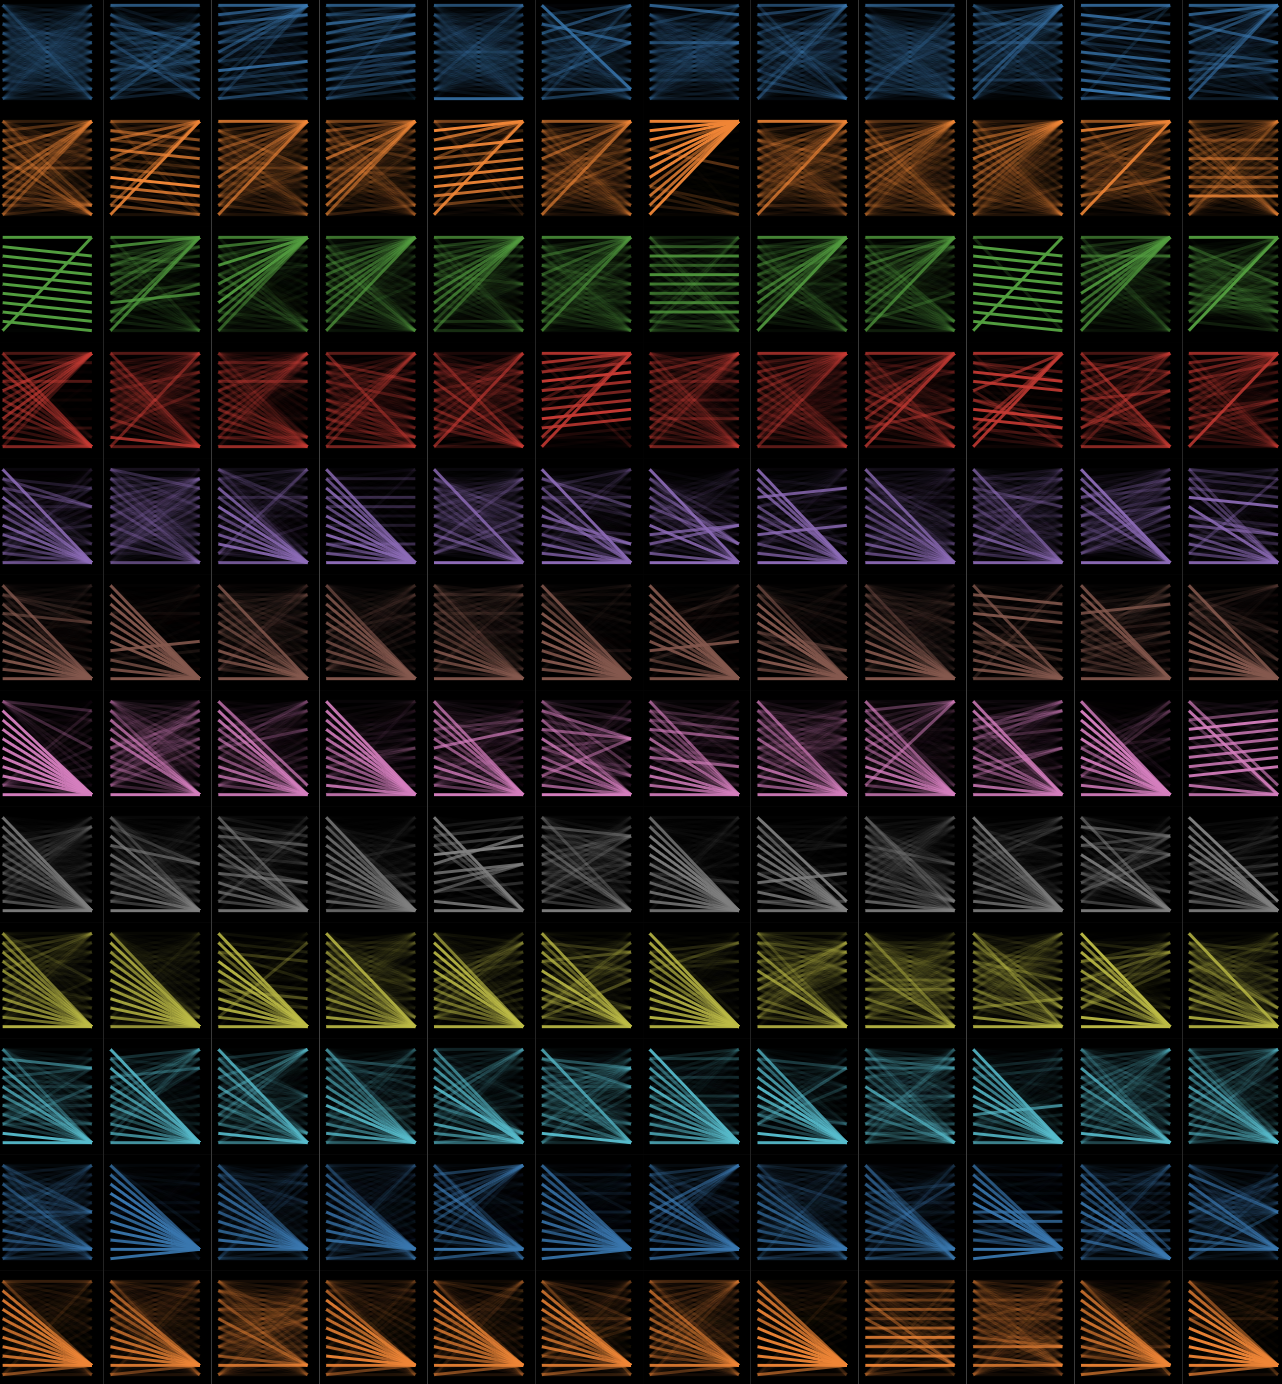
\includegraphics[width=\linewidth]{./image/bert_all.png}
    \caption{BERT ALL Layers\\
    (From top to bottom, is layer 0 to layer 11. From left to right, is the head 0 to head 8)}
  \label{bert_all}
\end{figure}



\begin{figure}[h]
    \centering
    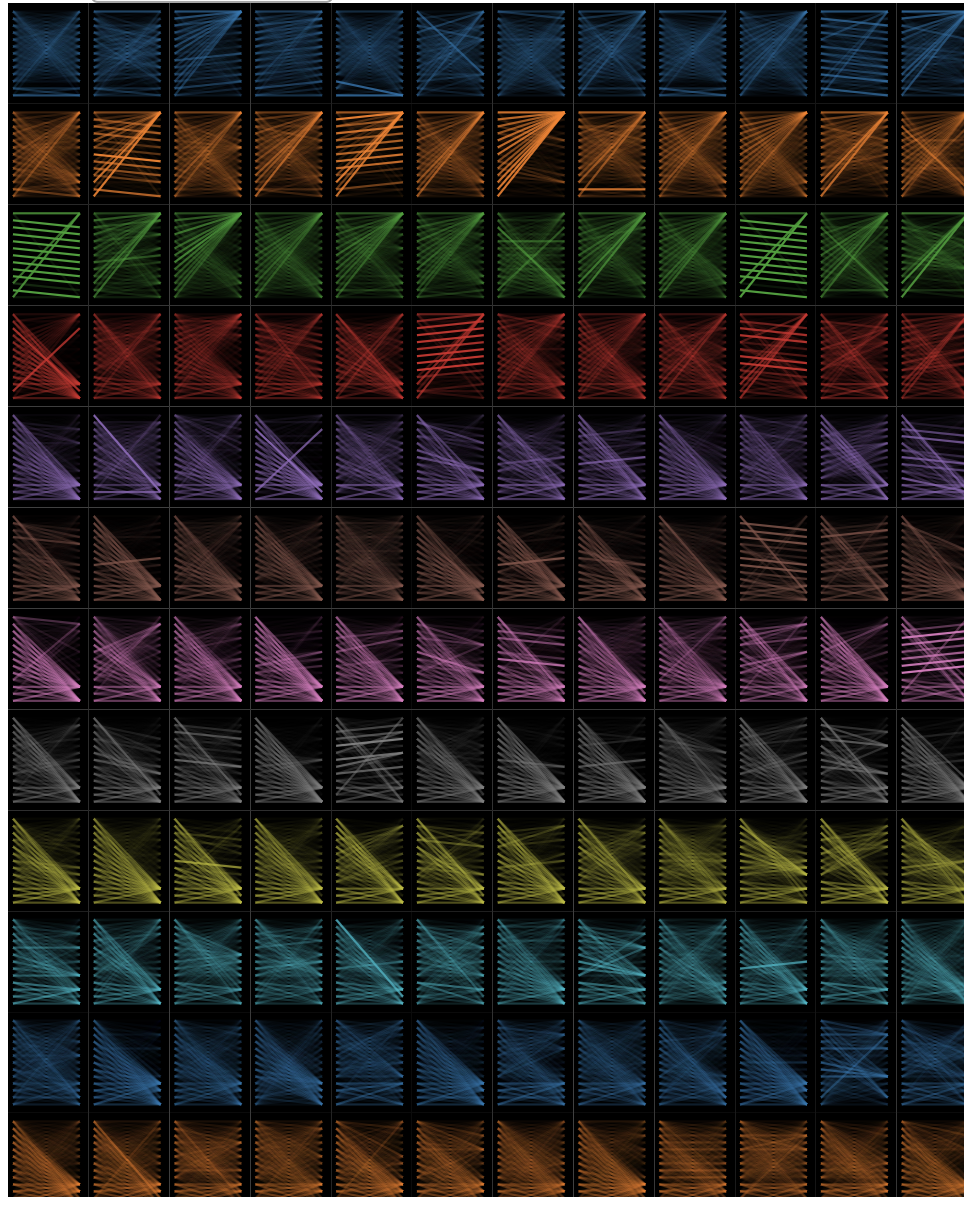
\includegraphics[width=\linewidth]{./image/spc_all.png}
    \caption{BERT-SPC ALL Layers\\
    (From top to bottom, is layer 0 to layer 11. From left to right, is the head 0 to head 8)}
  \label{spc_all}
\end{figure}






\chapter{Code}
Our code is available on \href{https://github.com/Xiang-Pan/TSA-PyTorch}{TSA-Pytorch}.

\end{document}
